\documentclass{beamer}

\usepackage[T1]{fontenc}
\usepackage[utf8]{inputenc}
\usepackage[frenchb]{babel}
\usepackage{pslatex}
\usepackage{colortbl}
\usepackage{calc}

\usetheme{Warsaw}


\definecolor{fondtitre}{rgb}{0.20,0.43,0.09}  % vert fonce
\definecolor{coultitre}{rgb}{0.41,0.05,0.05}  % marron
\definecolor{fondtexte}{rgb}{1,0.95,0.86}     % ivoire
\definecolor{autre1}{RGB}{250,150,5}  %vieux mauve
\definecolor{autre2}{RGB}{235,175,235} %horrible r
\colorlet{coultexte}{black}


\setbeamercolor{structure}{fg=coultitre, bg=fondtitre!40}
\setbeamercolor{block body}{bg=fondtexte}
\setbeamercolor{normal text}{fg=coultexte,bg=fondtexte}


\setbeamertemplate{footline}{
  \hbox{
    \hspace*{-0.06cm}

    \begin{beamercolorbox}[wd=.3\paperwidth,ht=2.25ex,dp=1ex,center]{title in head/foot}%
      \usebeamerfont{author in head/foot}\insertshortauthor
    \end{beamercolorbox}%

    \begin{beamercolorbox}[wd=.4\paperwidth,ht=2.25ex,dp=1ex,center]{title in head/foot}%
      \usebeamerfont{title in head/foot}\insertshorttitle
    \end{beamercolorbox}%

    \begin{beamercolorbox}[wd=.1\paperwidth,ht=2.25ex,dp=1ex,center]{date in head/foot}%
      \usebeamerfont{date in head/foot}
      \insertframenumber{} / \inserttotalframenumber\hspace*{2ex}
    \end{beamercolorbox}%

    \begin{beamercolorbox}[wd=.2\paperwidth,ht=2.25ex,dp=1ex,center]{date in head/foot}%
      \usebeamerfont{date in head/foot}\insertdate
  \end{beamercolorbox}}%

  \vskip0pt%
}


%navigation bar
\setbeamertemplate{navigation symbols}{%
  \insertslidenavigationsymbol
  \insertframenavigationsymbol
  \insertsubsectionnavigationsymbol
  \insertsectionnavigationsymbol
  \insertdocnavigationsymbol
  \insertbackfindforwardnavigationsymbol
}



\title[SoC]{Présentation du Projet Étrange}
\author{Caroline, Florian, Samuel}
\institute{Télécom Paristech}
\date{\today}


%---------------------------------------
%---------------------------------------


\begin{document}

\begin{frame}
  \titlepage
\end{frame}



%------------------ Plan ---------------
\section*{Plan}
\frame{\frametitle{Plan} \small \tableofcontents}
%

%------------------ Gestion de la mémoire ------------
\section{Gestion de la mémoire}
\begin{frame}
\begin{figure}[!h]
\centering
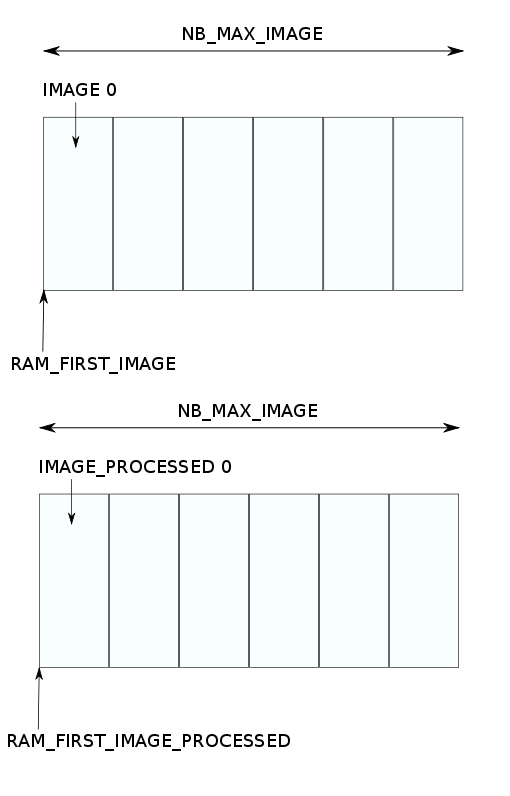
\includegraphics[scale = 0.23]{../rapport/ram_management.png}
\caption{ram management}
\end{figure}
\end{frame}

%------------------ Gestion du cache ------------
\section{Gestion du cache}
\begin{frame}
\begin{figure}[!h]
\centering
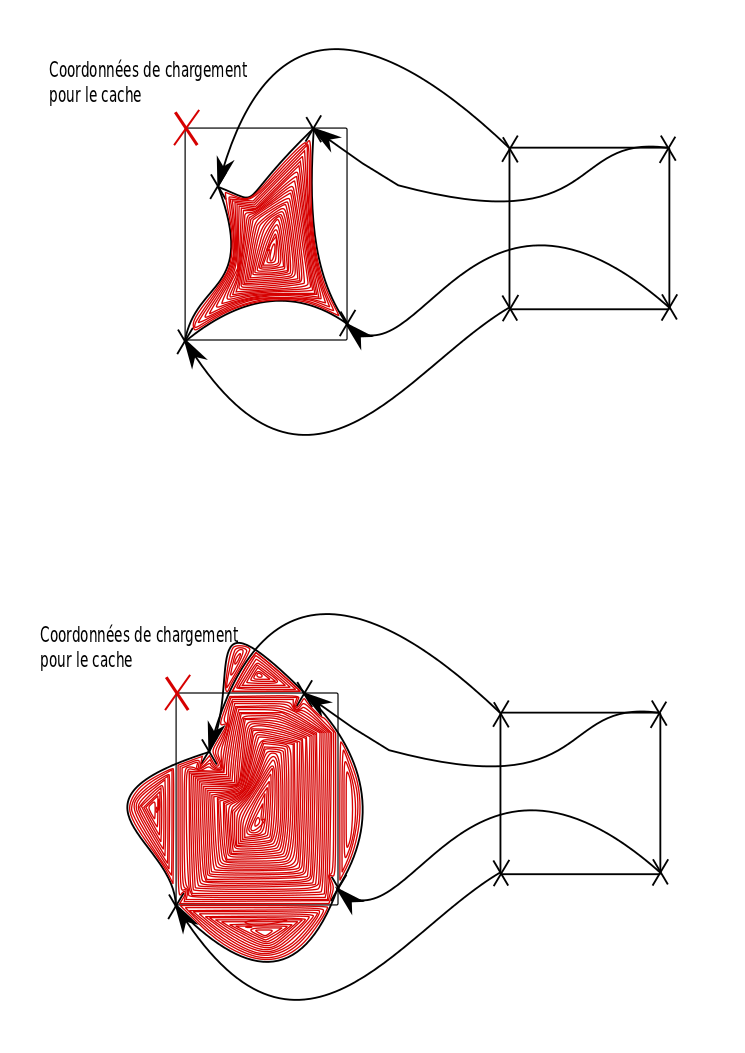
\includegraphics[scale = 0.18]{../rapport/cache_proc.png}
\caption{gestion du cache}
\end{figure}
\end{frame}


%------------------ Transfo : Rotation ------------
\section{Transfo : Rotation}
\begin{frame}
\begin{figure}[!h]
\centering
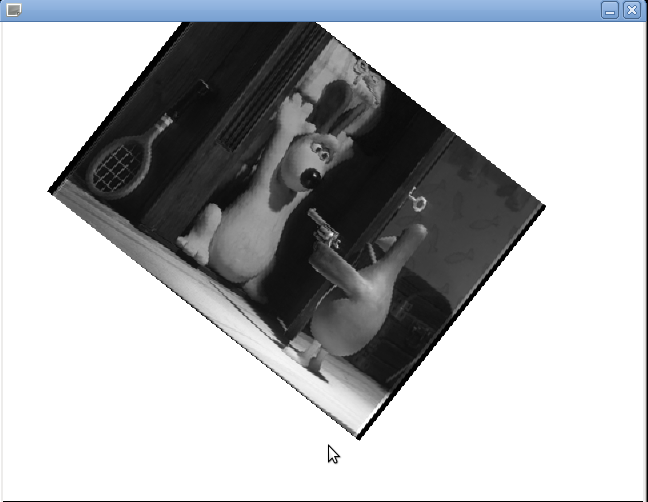
\includegraphics[scale = 0.3]{Rotation.png}
\caption{Transfo : rotation}
\end{figure}
\end{frame}

%------------------ Transfo : Inversion ------------
\section{Transfo : Inversion}
\begin{frame}
\begin{figure}[!h]
\centering
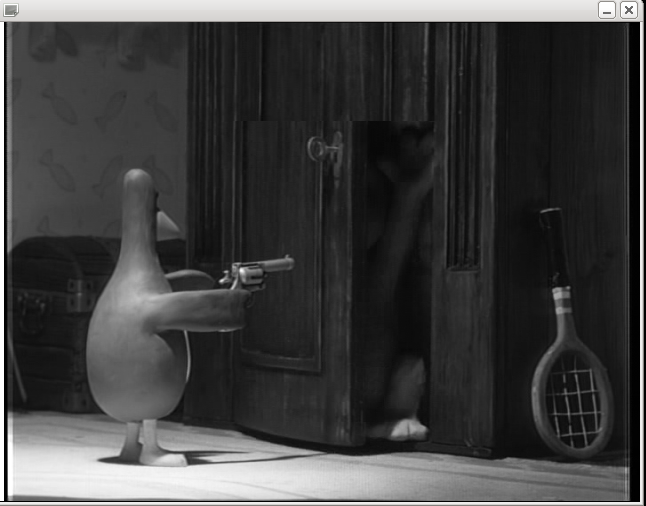
\includegraphics[scale = 0.3]{Inversion.png}
\caption{Transfo : inversion}
\end{figure}
\end{frame}

%------------------ Transfo : Ordre 2 ------------
\section{Transfo : Ordre 2}
\begin{frame}
\begin{figure}[!h]
\centering
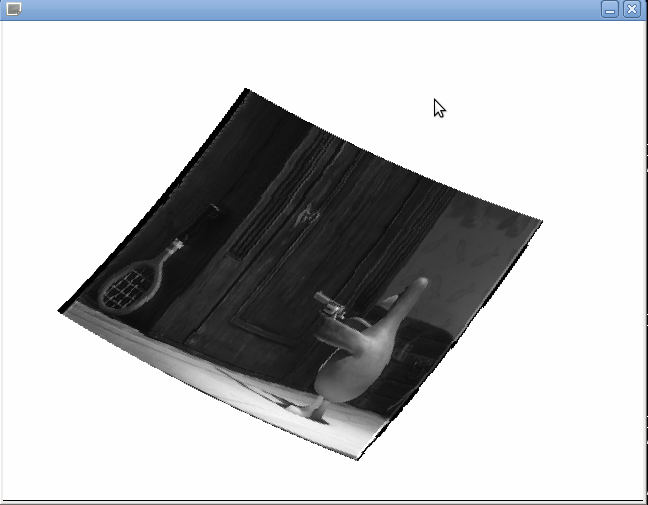
\includegraphics[scale = 0.3]{Transfo_ordre_2.png}
\caption{Transfo : Ordre 2}
\end{figure}
\end{frame}


%------------------ Transformation avec pb de cache ------------
\section{Transformation avec problème de cache (32*32)}
\begin{frame}
\begin{figure}[!h]
\centering
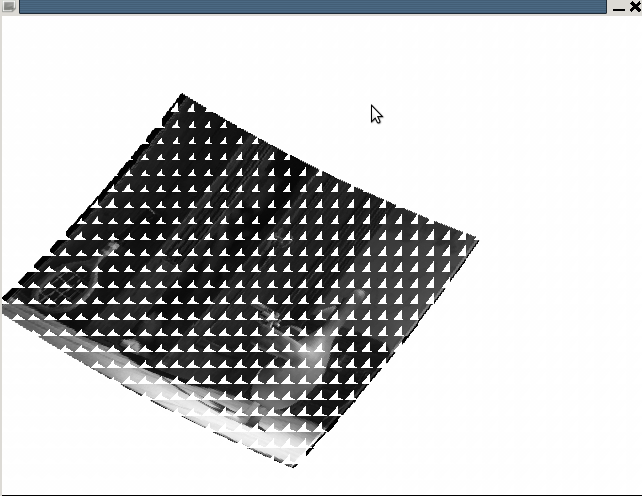
\includegraphics[scale = 0.3]{transfo_pb_cache.png}
\caption{Problème de cache (32*32)}
\end{figure}
\end{frame}

%------------------ Temps réel------------
\section{Temps réel}
\begin{frame}
\begin{figure}[!h]
\centering
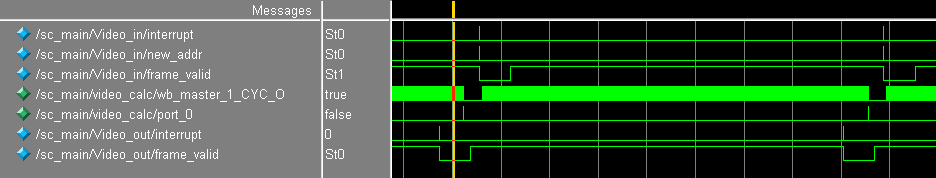
\includegraphics[scale = 0.3]{wave_r.png}
\caption{Avec un cache 48 bits et 4 temps pour lire dans la fifo}
\end{figure}
\end{frame}

\section{Temps réel}
\begin{frame}
\begin{figure}[!h]
\centering
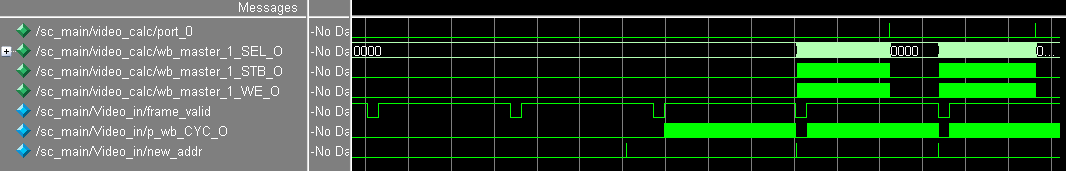
\includegraphics[scale = 0.3]{wave_cache32_r.png}
\caption{Avec un cache 32 bits et 4 temps pour lire dans la fifo}
\end{figure}
\end{frame}

\section{Temps réel}
\begin{frame}
\begin{figure}[!h]
\centering
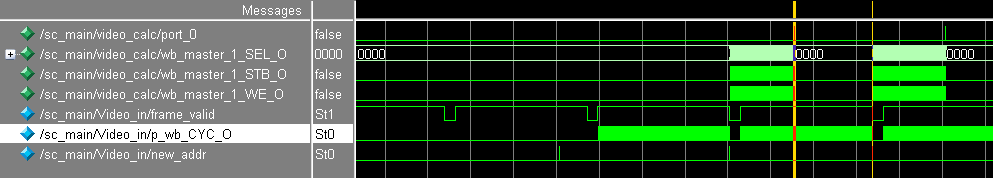
\includegraphics[scale = 0.3]{wave_sans_wait_r.png}
\caption{Avec un cache 48 bits et 1 temps pour lire dans la fifo}
\end{figure}
\end{frame}

%------------------ LES PSSC ------------
\section{PSSC}
\end{document}
